\documentclass[12pt,a4paper]{moderncv}

% moderncv themes
\moderncvtheme[red]{classic}                  % optional argument are 'blue' (default), 'orange', 'green', 'red', 'purple', 'grey' and 'roman' (for roman fonts, instead of sans serif fonts)

% character encoding
\usepackage[utf8]{vntex}                   % replace by the encoding you are using
\usepackage{bold-extra}

% adjust the page margins
\usepackage[scale=0.8]{geometry}
\setlength{\hintscolumnwidth}{3cm}						% if you want to change the width of the column with the dates
%\AtBeginDocument{\setlength{\maketitlenamewidth}{6cm}}  % only for the classic theme, if you want to change the width of your name placeholder (to leave more space for your address details
%\AtBeginDocument{\recomputelengths}                     % required when changes are made to page layout lengths

% personal data
\firstname{Duong}
\familyname{Bao Duy}
%\title{Curriculum Vitae}                      % optional, remove the line if not wanted
%\address{street and number}{postcode city}    % optional, remove the line if not wanted
%\mobile{mobile (optional)}                    % optional, remove the line if not wanted
%\phone{phone (optional)}                      % optional, remove the line if not wanted
%\fax{fax (optional)}                          % optional, remove the line if not wanted
%\email{email (optional)}                      % optional, remove the line if not wanted
%%\homepage{homepage (optional)}                % optional, remove the line if not wanted
%\extrainfo{additional information (optional)} % optional, remove the line if not wanted
%%\photo[64pt][0.4pt]{picture}                         % '64pt' is the height the picture must be resized to, 0.4pt is the thickness of the frame around it (put it to 0pt for no frame) and 'picture' is the name of the picture file; optional, remove the line if not wanted
%\quote{Some quote (optional)}                 % optional, remove the line if not wanted

% to show numerical labels in the bibliography; only useful if you make citations in your resume
%\makeatletter
%%\renewcommand*{\bibliographyitemlabel}{\@biblabel{\arabic{enumiv}}}
%\makeatother

% bibliography with mutiple entries
%\usepackage{multibib}
%\newcites{book,misc}{{Books},{Others}}

%\nopagenumbers{}                             % uncomment to suppress automatic page numbering for CVs longer than one page
%----------------------------------------------------------------------------------
%            content
%----------------------------------------------------------------------------------
\newcommand{\phongsection}[2]{\textrm{{\Large #1}}\textrm{{\normalsize #2}}}
\newcommand{\cvlined}[2]{\cvline{\footnotesize{#1}}{#2}}

%\newfont{\newnamef}{timenrb at 12pt}
\begin{document}
%\maketitle
\begin{flushright}
\textcolor{black}{\fbox{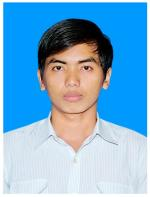
\includegraphics[scale=0.6]{pictures/picture.jpg}}}
\end{flushright}
\vspace*{-4.0cm}
\begin{Huge}
\textsc{Curriculum Vitae}
%\textbf{\phongsection{C}{URRICULUM} \phongsection{V}{ITAE}}
\end{Huge}
\vspace*{0.75cm}

\section{\textbf{\phongsection{P}{ERSONAL} \phongsection{I}{NFORMATION}}}
\vspace*{0.25cm}
\cvlined{Full Name}{\textbf{\phongsection{D}{UONG} \phongsection{B}{AO} \phongsection{D}{UY}}}
\cvlined{Sex}{Male}
\cvlined{Date of Brith}{Aug $22^{th}$, 1989.}
\cvlined{Place of Birth}{Ben Tre city, Vietnam.}
\cvlined{Home Address}{62/7/40D Nguyen Dinh Chinh, Dist.Phu Nhuan, Ho Chi Minh City, Vietnam}
\cvlined{Marital Status}{Single}
\cvlined{Email}{\href{mailto:baoduy.duong0206@gmail.com}{\underline{baoduy.duong0206@gmail.com}}}
\cvlined{Yahoo}{\href{ymsgr:baoduy\_duong0206@yahoo.com}{\underline{baoduy\_duong0206}}}
%\cvlined{Yahoo}{\href{mailto:baoduy_duong0206@yahoo.com}{\underline{baoduy_duong0206}}}
\cvlined{Phone number}{+84 1656-405-505}
\cvlined{Social network}{\begin{flushleft}
\href{https://www.facebook.com/baoduy.duong0206}{
\includegraphics[scale=0.4]{pictures/fb.png}}
\href{https://www.linkedin.com/in/baoduyduong}{
\includegraphics[scale=0.5]{pictures/linkin.png}}
\href{https://twitter.com/duong_bao_duy}{
\includegraphics[scale=0.5]{pictures/twitter.png}}
\href{https://plus.google.com/u/0/117631351363463841416/about}{
\includegraphics[scale=0.4]{pictures/g+.png}}
\end{flushleft}}
\cvlined{About me}{I am a programmer with 3+ years experience in Android development. Special, I have a solid skill about the linux system. So, I am happy working friendly or in a close team environment, and apply a positive attitude to every task undertake. And, I hope I can  create the application that will make user happy.}
\section{\textbf{\phongsection{B}{RIEF} \phongsection{M}{YSELF}}}
\cvlined{8/2013 – present}{ working at \href{http://www.bravesoft.vn/}{\underline{\textbf{BraveSoft Vietnam}}}}
\cvlined{4/2011– 2013}{ worked at \href{http://anttek.com/}{\underline{\textbf{AntTek}}}}
\cvlined{2007 – 5/2013}{have studied at Science University }
\cvlined{2010 – 8/2010}{studied at CCNA at Trung Tam Tin Hoc DHKHTN }
\cvlined{2004 – 2007}{studied at Ben Tre major high school}
\section{\textbf{\phongsection{K}{EY} \phongsection{S}{KILLS}}}
\cvlined{JAVA  }{Expert}
\cvlined{C/C++}{High}
\cvlined{UX}{High}
\cvlined{Network System}{High}
\cvlined{Linux System}{High}
\cvlined{OBJECTIVE-C}{Medium}
\cvlined{Opengl ES}{Medium}
\section{\textbf{\phongsection{S}{OFT} \phongsection{S}{KILLS}}}
\cvlined{• }{Time management with getting thing done (GTD) methodology}
\cvlined{• }{Public speaking}
\cvlined{• }{Conversation}
\cvlined{• }{Self motivation and organisation}
\section{\textbf{\phongsection{O}{THER} \phongsection{S}{KILLS}}}
\cvlined{Programming     
languages}{\textsc{Bash script}, \textsc{Pascal}, \textsc{Assembler}, \textsc{Javascript}, \textsc{html/css}, \textsc{python}, \LaTeX, \textsc{Lua}}
\cvlined{ Operating       
Systems}{*nix system, Window system, Hadoop ecosystem}
\cvlined{Databases       }{MS Access, MySql 5.0, MongoDB}
\cvlined{Miscellaneous tools}{Matlab, Maple, OpenOffice.org, Microsoft Office, Eclipse, Skype, Yahoo! Messenger, GNU tools}
\section{\textbf{\phongsection{L}{ANGUAGES}}}
\cvitemwithcomment{English}{Intermediate}{Read and listen fluently}
\cvitemwithcomment{Japanses}{Basic}{Basic words and phrases only}
\section{\textbf{\phongsection{A}{WARDS}}}
\cvlined{}{CCNA certified by Trung Tam Tin Hoc DHKHTN}
\section{\textbf{\phongsection{E}{MPLOYMENT} \phongsection{H}{ISTORY}}}
\cventry{}{\phongsection{A}{NDROID} \phongsection{D}{EVELOPER}}{}{}{}{BraveSoft Vietnam}
\cvlined{•  }{SynchroLife}
\cvlined{   }{- layout UI follow the specified.}
\cvlined{   }{- Analysis the api of server and write document.}
\cvlined{•  }{Take5ive}
\cvlined{   }{- layout UI follow the example application.}
\cvlined{   }{- Conceptualized, analysis the function of the example application, then implement on the current application.}
\cvlined{   }{- build ffmpeg on arm system with ndk.}
\vspace*{1.0cm}
\cventry{}{\phongsection{A}{NDROID} \phongsection{D}{EVELOPER}}{}{}{}{AntTek}
\cvlined{•  }{AntTek Explorer}
\cvlined{•  }{Pdf/Tiff module for AntTek Explorer}
\cvlined{•  }{Various of project need integrate network modules or get data from native code (JNI).}
\cvlined{•  }{Research about the contribution of Android source framework from repo. Build some ROM to test on real devices.}
\cvlined{•  }{Rooting some Android devices: Galaxy S, Nook Color, Kindle fire, ...}
\vspace*{1.0cm}
\cventry{}{\phongsection{C}{ONTRIBUTOR} \phongsection{O}{F} \phongsection{O}{PEN SOURCE}}{}{}{}{}
\cvlined{•  }{Had join to some projects, such as: android-anpr,openintents, Android-Flash-P2P,..., of course, as the role of forker.}
\end{document}